\documentclass[oneside, 12pt, a4paper]{article}
\usepackage[utf8]{inputenc} 
\usepackage[T1]{fontenc} 
\usepackage{microtype} 
\usepackage{amsmath, amssymb, mathtools} 
\usepackage{graphicx} 
\usepackage{hyperref} 
\hypersetup{colorlinks=false,urlcolor=black} 
\usepackage{float}
\usepackage{listings}
\usepackage{lmodern}
\makeatletter
\title{Big Programming Exercise}    
\author{Qingyu Huang \\
201703956}        
\date{\today}                   
\makeatother

\begin{document}
\maketitle

\section*{Natural logarithm}
%
The natural logarithm of a real positive number x using the integral representation is:
%
\begin{align}
    \ln x=\int_1^x{\frac{1}{t}dt}
\end{align}
%
To reduce the logarithm of an arbitrary positive number to the logarithm of a number in the range $1\leqslant x<2$ using the formulae:
%
\begin{align}
    \ln x=-\ln \frac{1}{x} \\
    \ln x=\ln 2+\ln \frac{x}{2}
\end{align}
We divide $(\text{0,}+\infty) $ into 4 intervals:$(\text{0,}\frac{1}{2}) $, $(\frac{1}{2},1) $, $(\text{1,}2) $ and $(\text{2,}+\infty)$.\\
if $x\in (\text{0,}\frac{1}{2})$ then use formulae $\ln x=-\ln \frac{1}{x}$ to change x to $x \in (\text{2,}+\infty) $ then use formulae $\ln x=\ln 2+\ln \frac{x}{2}$ several times until change $x \in (\text{1,}2) $. for example:
\begin{align}
    \ln 10=\ln 2+\ln \frac{10}{2}=  2\ln 2+\ln \frac{10}{2^2}=  3 \ln2 + \ln \frac{10}{2^3}
\end{align}
else if $x\in (\frac{1}{2},1)$ then use formulae $\ln x=-\ln \frac{1}{x}$ to change x to $x \in (\text{1,}2)$.\\
else if $x\in (\text{2,}+\infty)$ then use formulae $\ln x=\ln 2+\ln \frac{x}{2}$ several times until change $x \in (\text{1,}2) $.


This is a numerical integration problem can be solved by using the GNU Scientific Library (GSL). First provide to function to integrate gsl\_function as $\frac{1}{x}$, then i use adaptive Gauss-Kronrod integrator fucntion gsl\_integration\_qag with 61 point Gauss-Kronrod rules to calculate the numerical integration, the lower bound a is 1 and the upper bound b is x, the desired absolute and relative error limits is 1e-8, the maximum number of subintervals is 1e3. Then in the main function, x ranges from 0.1 to 10.0 with step 0.2 was caculated, and print into a file called data, then use gnuplot with plot.gpi to plot the final result and compared with natural logarithm function from <math.h>.

\subsection*{Plot}

\begin{center}
    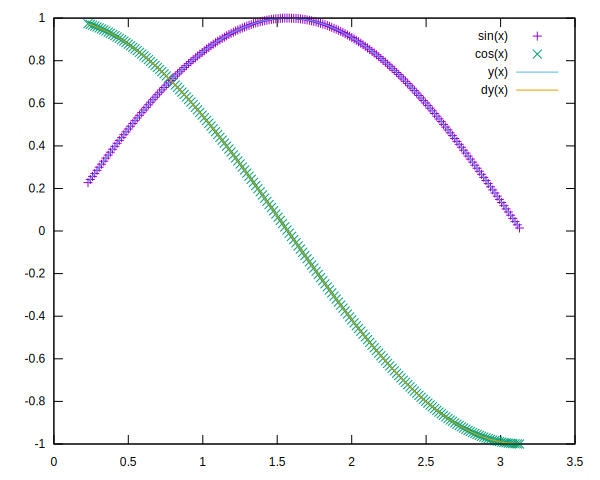
\includegraphics[width=1\textwidth]{plot.pdf}
\end{center}
%
As shown on the figure, the green curve is the result of natural logarithm function from \texttt{math.h}, the points with marker '+' is my natural logarithm with numerical integration, it's clear that they matches very well.  

\subsection*{References}
%
Galassi, M., et al. "GNU Scientific Library Reference Manual, ISBN 0954612078." Library available online at http://www.gnu.org/software/gsl (2015).

%\nocite{*} % printer hele bibliografien
%\printbibliography 
\end{document}
